\documentclass[twoside]{book}

% Packages required by doxygen
\usepackage{fixltx2e}
\usepackage{calc}
\usepackage{doxygen}
\usepackage[export]{adjustbox} % also loads graphicx
\usepackage{graphicx}
\usepackage[utf8]{inputenc}
\usepackage{makeidx}
\usepackage{multicol}
\usepackage{multirow}
\PassOptionsToPackage{warn}{textcomp}
\usepackage{textcomp}
\usepackage[nointegrals]{wasysym}
\usepackage[table]{xcolor}

% Font selection
\usepackage[T1]{fontenc}
\usepackage[scaled=.90]{helvet}
\usepackage{courier}
\usepackage{amssymb}
\usepackage{sectsty}
\renewcommand{\familydefault}{\sfdefault}
\allsectionsfont{%
  \fontseries{bc}\selectfont%
  \color{darkgray}%
}
\renewcommand{\DoxyLabelFont}{%
  \fontseries{bc}\selectfont%
  \color{darkgray}%
}
\newcommand{\+}{\discretionary{\mbox{\scriptsize$\hookleftarrow$}}{}{}}

% Page & text layout
\usepackage{geometry}
\geometry{%
  a4paper,%
  top=2.5cm,%
  bottom=2.5cm,%
  left=2.5cm,%
  right=2.5cm%
}
\tolerance=750
\hfuzz=15pt
\hbadness=750
\setlength{\emergencystretch}{15pt}
\setlength{\parindent}{0cm}
\setlength{\parskip}{3ex plus 2ex minus 2ex}
\makeatletter
\renewcommand{\paragraph}{%
  \@startsection{paragraph}{4}{0ex}{-1.0ex}{1.0ex}{%
    \normalfont\normalsize\bfseries\SS@parafont%
  }%
}
\renewcommand{\subparagraph}{%
  \@startsection{subparagraph}{5}{0ex}{-1.0ex}{1.0ex}{%
    \normalfont\normalsize\bfseries\SS@subparafont%
  }%
}
\makeatother

% Headers & footers
\usepackage{fancyhdr}
\pagestyle{fancyplain}
\fancyhead[LE]{\fancyplain{}{\bfseries\thepage}}
\fancyhead[CE]{\fancyplain{}{}}
\fancyhead[RE]{\fancyplain{}{\bfseries\leftmark}}
\fancyhead[LO]{\fancyplain{}{\bfseries\rightmark}}
\fancyhead[CO]{\fancyplain{}{}}
\fancyhead[RO]{\fancyplain{}{\bfseries\thepage}}
\fancyfoot[LE]{\fancyplain{}{}}
\fancyfoot[CE]{\fancyplain{}{}}
\fancyfoot[RE]{\fancyplain{}{\bfseries\scriptsize Generated by Doxygen }}
\fancyfoot[LO]{\fancyplain{}{\bfseries\scriptsize Generated by Doxygen }}
\fancyfoot[CO]{\fancyplain{}{}}
\fancyfoot[RO]{\fancyplain{}{}}
\renewcommand{\footrulewidth}{0.4pt}
\renewcommand{\chaptermark}[1]{%
  \markboth{#1}{}%
}
\renewcommand{\sectionmark}[1]{%
  \markright{\thesection\ #1}%
}

% Indices & bibliography
\usepackage{natbib}
\usepackage[titles]{tocloft}
\setcounter{tocdepth}{3}
\setcounter{secnumdepth}{5}
\makeindex

% Hyperlinks (required, but should be loaded last)
\usepackage{ifpdf}
\ifpdf
  \usepackage[pdftex,pagebackref=true]{hyperref}
\else
  \usepackage[ps2pdf,pagebackref=true]{hyperref}
\fi
\hypersetup{%
  colorlinks=true,%
  linkcolor=blue,%
  citecolor=blue,%
  unicode%
}

% Custom commands
\newcommand{\clearemptydoublepage}{%
  \newpage{\pagestyle{empty}\cleardoublepage}%
}

\usepackage{caption}
\captionsetup{labelsep=space,justification=centering,font={bf},singlelinecheck=off,skip=4pt,position=top}

%===== C O N T E N T S =====

\begin{document}

% Titlepage & ToC
\hypersetup{pageanchor=false,
             bookmarksnumbered=true,
             pdfencoding=unicode
            }
\pagenumbering{alph}
\begin{titlepage}
\vspace*{7cm}
\begin{center}%
{\Large My Project }\\
\vspace*{1cm}
{\large Generated by Doxygen 1.8.14}\\
\end{center}
\end{titlepage}
\clearemptydoublepage
\pagenumbering{roman}
\tableofcontents
\clearemptydoublepage
\pagenumbering{arabic}
\hypersetup{pageanchor=true}

%--- Begin generated contents ---
\chapter{Hierarchical Index}
\section{Class Hierarchy}
This inheritance list is sorted roughly, but not completely, alphabetically\+:\begin{DoxyCompactList}
\item \contentsline{section}{Calibration\+\_\+\+Instrinsic}{\pageref{class_calibration___instrinsic}}{}
\item \contentsline{section}{Cell}{\pageref{class_cell}}{}
\item \contentsline{section}{Character\+\_\+\+Recognition\+\_\+\+Algorithm}{\pageref{class_character___recognition___algorithm}}{}
\begin{DoxyCompactList}
\item \contentsline{section}{Optical\+\_\+\+Character\+\_\+\+Recognition}{\pageref{class_optical___character___recognition}}{}
\item \contentsline{section}{Template\+\_\+\+Character\+\_\+\+Recognition}{\pageref{class_template___character___recognition}}{}
\end{DoxyCompactList}
\item \contentsline{section}{Clipper}{\pageref{class_clipper}}{}
\item \contentsline{section}{Path\+Finder\+:\+:Collision\+Detector}{\pageref{class_path_finder_1_1_collision_detector}}{}
\item \contentsline{section}{Color\+\_\+\+Processing}{\pageref{class_color___processing}}{}
\item \contentsline{section}{Digit\+\_\+\+Recognition}{\pageref{class_digit___recognition}}{}
\item \contentsline{section}{Digit\+Result\+Distribution}{\pageref{struct_digit_result_distribution}}{}
\item \contentsline{section}{H\+S\+V\+Filter\+Range}{\pageref{struct_h_s_v_filter_range}}{}
\item \contentsline{section}{Inverse\+\_\+\+Perspective\+\_\+\+Mapping}{\pageref{class_inverse___perspective___mapping}}{}
\item \contentsline{section}{Line}{\pageref{class_line}}{}
\begin{DoxyCompactList}
\item \contentsline{section}{Circular\+Line}{\pageref{class_circular_line}}{}
\item \contentsline{section}{Straight\+Line}{\pageref{class_straight_line}}{}
\end{DoxyCompactList}
\item \contentsline{section}{Map}{\pageref{class_map}}{}
\item \contentsline{section}{Path}{\pageref{class_path}}{}
\item \contentsline{section}{Path\+Coordinates}{\pageref{class_path_coordinates}}{}
\item \contentsline{section}{Path\+Finder}{\pageref{class_path_finder}}{}
\begin{DoxyCompactList}
\item \contentsline{section}{Dubin\+Path\+Finder}{\pageref{class_dubin_path_finder}}{}
\end{DoxyCompactList}
\item \contentsline{section}{People\+Storage}{\pageref{struct_people_storage}}{}
\item \contentsline{section}{Position}{\pageref{class_position}}{}
\item \contentsline{section}{Dubin\+Path\+Finder\+:\+:Possible\+Dubin\+Path}{\pageref{class_dubin_path_finder_1_1_possible_dubin_path}}{}
\item \contentsline{section}{Settings}{\pageref{class_settings}}{}
\item \contentsline{section}{Shape}{\pageref{class_shape}}{}
\begin{DoxyCompactList}
\item \contentsline{section}{Circle}{\pageref{class_circle}}{}
\begin{DoxyCompactList}
\item \contentsline{section}{People}{\pageref{class_people}}{}
\item \contentsline{section}{Robot}{\pageref{class_robot}}{}
\end{DoxyCompactList}
\item \contentsline{section}{Obstacle}{\pageref{class_obstacle}}{}
\item \contentsline{section}{Polygon}{\pageref{class_polygon}}{}
\begin{DoxyCompactList}
\item \contentsline{section}{Hexagon}{\pageref{class_hexagon}}{}
\item \contentsline{section}{Pentagon}{\pageref{class_pentagon}}{}
\item \contentsline{section}{Rectangle}{\pageref{class_rectangle}}{}
\begin{DoxyCompactList}
\item \contentsline{section}{Arena}{\pageref{class_arena}}{}
\item \contentsline{section}{Exit\+Point}{\pageref{class_exit_point}}{}
\item \contentsline{section}{Square}{\pageref{class_square}}{}
\end{DoxyCompactList}
\item \contentsline{section}{Triangle}{\pageref{class_triangle}}{}
\end{DoxyCompactList}
\end{DoxyCompactList}
\item \contentsline{section}{standard\+Conf}{\pageref{structstandard_conf}}{}
\item \contentsline{section}{Undistorsion}{\pageref{class_undistorsion}}{}
\end{DoxyCompactList}

\chapter{Class Index}
\section{Class List}
Here are the classes, structs, unions and interfaces with brief descriptions\+:\begin{DoxyCompactList}
\item\contentsline{section}{\mbox{\hyperlink{class_arena}{Arena}} }{\pageref{class_arena}}{}
\item\contentsline{section}{\mbox{\hyperlink{class_calibration___instrinsic}{Calibration\+\_\+\+Instrinsic}} }{\pageref{class_calibration___instrinsic}}{}
\item\contentsline{section}{\mbox{\hyperlink{class_cell}{Cell}} }{\pageref{class_cell}}{}
\item\contentsline{section}{\mbox{\hyperlink{class_character___recognition___algorithm}{Character\+\_\+\+Recognition\+\_\+\+Algorithm}} \\*Abstract class for character recognition algorithms }{\pageref{class_character___recognition___algorithm}}{}
\item\contentsline{section}{\mbox{\hyperlink{class_circle}{Circle}} }{\pageref{class_circle}}{}
\item\contentsline{section}{\mbox{\hyperlink{class_color___processing}{Color\+\_\+\+Processing}} }{\pageref{class_color___processing}}{}
\item\contentsline{section}{\mbox{\hyperlink{class_digit___recognition}{Digit\+\_\+\+Recognition}} \\*Used to detect digits in the arena and export \mbox{\hyperlink{struct_people_data}{People\+Data}} }{\pageref{class_digit___recognition}}{}
\item\contentsline{section}{\mbox{\hyperlink{struct_digit_result_distribution}{Digit\+Result\+Distribution}} }{\pageref{struct_digit_result_distribution}}{}
\item\contentsline{section}{\mbox{\hyperlink{class_exit_point}{Exit\+Point}} }{\pageref{class_exit_point}}{}
\item\contentsline{section}{\mbox{\hyperlink{class_hexagon}{Hexagon}} }{\pageref{class_hexagon}}{}
\item\contentsline{section}{\mbox{\hyperlink{struct_h_s_v_filter_range}{H\+S\+V\+Filter\+Range}} }{\pageref{struct_h_s_v_filter_range}}{}
\item\contentsline{section}{\mbox{\hyperlink{class_image___processing}{Image\+\_\+\+Processing}} }{\pageref{class_image___processing}}{}
\item\contentsline{section}{\mbox{\hyperlink{class_inverse___perspective___mapping}{Inverse\+\_\+\+Perspective\+\_\+\+Mapping}} }{\pageref{class_inverse___perspective___mapping}}{}
\item\contentsline{section}{\mbox{\hyperlink{class_map}{Map}} }{\pageref{class_map}}{}
\item\contentsline{section}{\mbox{\hyperlink{class_obstacle}{Obstacle}} }{\pageref{class_obstacle}}{}
\item\contentsline{section}{\mbox{\hyperlink{class_optical___character___recognition}{Optical\+\_\+\+Character\+\_\+\+Recognition}} \\*O\+CP algorithm from tesseract library }{\pageref{class_optical___character___recognition}}{}
\item\contentsline{section}{\mbox{\hyperlink{class_pentagon}{Pentagon}} }{\pageref{class_pentagon}}{}
\item\contentsline{section}{\mbox{\hyperlink{class_people}{People}} }{\pageref{class_people}}{}
\item\contentsline{section}{\mbox{\hyperlink{struct_people_data}{People\+Data}} \\*Data object that is beeing used to build a \mbox{\hyperlink{class_people}{People}} Object for the map representation }{\pageref{struct_people_data}}{}
\item\contentsline{section}{\mbox{\hyperlink{class_settings}{Settings}} }{\pageref{class_settings}}{}
\item\contentsline{section}{\mbox{\hyperlink{class_shape}{Shape}} }{\pageref{class_shape}}{}
\item\contentsline{section}{\mbox{\hyperlink{class_square}{Square}} }{\pageref{class_square}}{}
\item\contentsline{section}{\mbox{\hyperlink{class_template___character___recognition}{Template\+\_\+\+Character\+\_\+\+Recognition}} }{\pageref{class_template___character___recognition}}{}
\item\contentsline{section}{\mbox{\hyperlink{class_triangle}{Triangle}} }{\pageref{class_triangle}}{}
\item\contentsline{section}{\mbox{\hyperlink{class_undistorsion}{Undistorsion}} }{\pageref{class_undistorsion}}{}
\item\contentsline{section}{\mbox{\hyperlink{struct_user_data}{User\+Data}} }{\pageref{struct_user_data}}{}
\end{DoxyCompactList}

\chapter{Class Documentation}
\hypertarget{class_circular_line}{}\section{Circular\+Line Class Reference}
\label{class_circular_line}\index{Circular\+Line@{Circular\+Line}}


Class for managing circle in the pat.  




{\ttfamily \#include $<$Circular\+Line.\+hpp$>$}

Inheritance diagram for Circular\+Line\+:\begin{figure}[H]
\begin{center}
\leavevmode
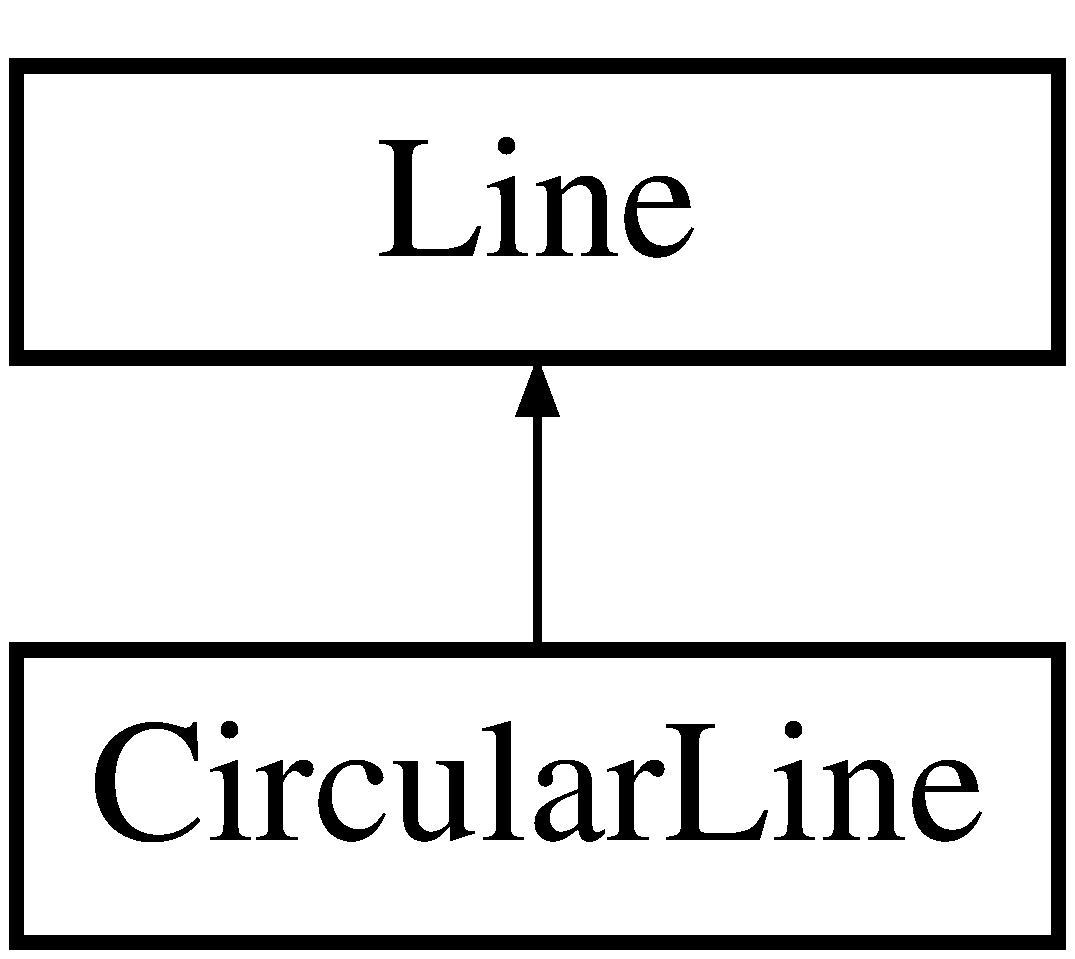
\includegraphics[height=2.000000cm]{class_circular_line}
\end{center}
\end{figure}
\subsection*{Public Member Functions}
\begin{DoxyCompactItemize}
\item 
\mbox{\hyperlink{class_circular_line_aacb17f31ed3eb9fbe66fbe2a95b20e6a}{Circular\+Line}} (\mbox{\hyperlink{class_position}{Position}} start\+\_\+point, double curvature, double length)
\begin{DoxyCompactList}\small\item\em constructor of the class \end{DoxyCompactList}\item 
\mbox{\Hypertarget{class_circular_line_a2f8c59281cb51a6072b6980b6df9be89}\label{class_circular_line_a2f8c59281cb51a6072b6980b6df9be89}} 
\mbox{\hyperlink{class_circular_line_a2f8c59281cb51a6072b6980b6df9be89}{$\sim$\+Circular\+Line}} ()
\begin{DoxyCompactList}\small\item\em destructor of the class \end{DoxyCompactList}\item 
\mbox{\Hypertarget{class_circular_line_a521ac7d10eca4ea8914465c5eea90d8d}\label{class_circular_line_a521ac7d10eca4ea8914465c5eea90d8d}} 
void \mbox{\hyperlink{class_circular_line_a521ac7d10eca4ea8914465c5eea90d8d}{set\+Curvature}} (double curvature\+\_\+i)
\begin{DoxyCompactList}\small\item\em allow to set the curvature of the line \end{DoxyCompactList}\item 
double \mbox{\hyperlink{class_circular_line_ab5bad8246cee1a80c1e625c68c0b2c15}{get\+Curvature}} ()
\end{DoxyCompactItemize}


\subsection{Detailed Description}
Class for managing circle in the pat. 

\subsection{Constructor \& Destructor Documentation}
\mbox{\Hypertarget{class_circular_line_aacb17f31ed3eb9fbe66fbe2a95b20e6a}\label{class_circular_line_aacb17f31ed3eb9fbe66fbe2a95b20e6a}} 
\index{Circular\+Line@{Circular\+Line}!Circular\+Line@{Circular\+Line}}
\index{Circular\+Line@{Circular\+Line}!Circular\+Line@{Circular\+Line}}
\subsubsection{\texorpdfstring{Circular\+Line()}{CircularLine()}}
{\footnotesize\ttfamily Circular\+Line\+::\+Circular\+Line (\begin{DoxyParamCaption}\item[{\mbox{\hyperlink{class_position}{Position}}}]{start\+\_\+point,  }\item[{double}]{curvature,  }\item[{double}]{length }\end{DoxyParamCaption})}



constructor of the class 


\begin{DoxyParams}{Parameters}
{\em start\+\_\+point} & start position of the line \\
\hline
{\em curvature} & curvature of the path \\
\hline
{\em length} & length of the path \\
\hline
\end{DoxyParams}


\subsection{Member Function Documentation}
\mbox{\Hypertarget{class_circular_line_ab5bad8246cee1a80c1e625c68c0b2c15}\label{class_circular_line_ab5bad8246cee1a80c1e625c68c0b2c15}} 
\index{Circular\+Line@{Circular\+Line}!get\+Curvature@{get\+Curvature}}
\index{get\+Curvature@{get\+Curvature}!Circular\+Line@{Circular\+Line}}
\subsubsection{\texorpdfstring{get\+Curvature()}{getCurvature()}}
{\footnotesize\ttfamily double Circular\+Line\+::get\+Curvature (\begin{DoxyParamCaption}{ }\end{DoxyParamCaption})}

return the curvature of the line \begin{DoxyReturn}{Returns}
curvature of the line 
\end{DoxyReturn}


The documentation for this class was generated from the following file\+:\begin{DoxyCompactItemize}
\item 
Circular\+Line.\+hpp\end{DoxyCompactItemize}

\hypertarget{class_dubin_path}{}\section{Dubin\+Path Class Reference}
\label{class_dubin_path}\index{Dubin\+Path@{Dubin\+Path}}


Class that given the path coordinates allow to find the path using the dubins path algorithm.  




{\ttfamily \#include $<$Dubin\+Path.\+hpp$>$}

\subsection*{Public Member Functions}
\begin{DoxyCompactItemize}
\item 
\mbox{\hyperlink{class_dubin_path_a095a22d8f3c9780b09fc1e48be9011b3}{Dubin\+Path}} (\mbox{\hyperlink{class_path_coordinates}{Path\+Coordinates}} path\+\_\+coordinates\+\_\+i)
\begin{DoxyCompactList}\small\item\em constructor of the \mbox{\hyperlink{class_dubin_path}{Dubin\+Path}} class \end{DoxyCompactList}\item 
\mbox{\Hypertarget{class_dubin_path_a89b962b8ff3bf5cbb9fda6d539bb7a9c}\label{class_dubin_path_a89b962b8ff3bf5cbb9fda6d539bb7a9c}} 
\mbox{\hyperlink{class_dubin_path_a89b962b8ff3bf5cbb9fda6d539bb7a9c}{$\sim$\+Dubin\+Path}} ()
\begin{DoxyCompactList}\small\item\em destructor of the \mbox{\hyperlink{class_dubin_path}{Dubin\+Path}} class \end{DoxyCompactList}\item 
std\+::vector$<$ \mbox{\hyperlink{class_line}{Line}} $>$ \mbox{\hyperlink{class_dubin_path_a260513ceab4e25a5a8867ea2701fbb68}{dubin\+Shortest\+Path}} ()
\begin{DoxyCompactList}\small\item\em function that find the dubins shortest path and return a vector of line \end{DoxyCompactList}\end{DoxyCompactItemize}


\subsection{Detailed Description}
Class that given the path coordinates allow to find the path using the dubins path algorithm. 

\subsection{Constructor \& Destructor Documentation}
\mbox{\Hypertarget{class_dubin_path_a095a22d8f3c9780b09fc1e48be9011b3}\label{class_dubin_path_a095a22d8f3c9780b09fc1e48be9011b3}} 
\index{Dubin\+Path@{Dubin\+Path}!Dubin\+Path@{Dubin\+Path}}
\index{Dubin\+Path@{Dubin\+Path}!Dubin\+Path@{Dubin\+Path}}
\subsubsection{\texorpdfstring{Dubin\+Path()}{DubinPath()}}
{\footnotesize\ttfamily Dubin\+Path\+::\+Dubin\+Path (\begin{DoxyParamCaption}\item[{\mbox{\hyperlink{class_path_coordinates}{Path\+Coordinates}}}]{path\+\_\+coordinates\+\_\+i }\end{DoxyParamCaption})}



constructor of the \mbox{\hyperlink{class_dubin_path}{Dubin\+Path}} class 


\begin{DoxyParams}{Parameters}
{\em path\+\_\+coordinates\+\_\+i} & coordinates of the path that we want to find \\
\hline
\end{DoxyParams}


\subsection{Member Function Documentation}
\mbox{\Hypertarget{class_dubin_path_a260513ceab4e25a5a8867ea2701fbb68}\label{class_dubin_path_a260513ceab4e25a5a8867ea2701fbb68}} 
\index{Dubin\+Path@{Dubin\+Path}!dubin\+Shortest\+Path@{dubin\+Shortest\+Path}}
\index{dubin\+Shortest\+Path@{dubin\+Shortest\+Path}!Dubin\+Path@{Dubin\+Path}}
\subsubsection{\texorpdfstring{dubin\+Shortest\+Path()}{dubinShortestPath()}}
{\footnotesize\ttfamily std\+::vector$<$\mbox{\hyperlink{class_line}{Line}}$>$ Dubin\+Path\+::dubin\+Shortest\+Path (\begin{DoxyParamCaption}{ }\end{DoxyParamCaption})}



function that find the dubins shortest path and return a vector of line 

\begin{DoxyReturn}{Returns}
vector of lines which describes the path 
\end{DoxyReturn}


The documentation for this class was generated from the following file\+:\begin{DoxyCompactItemize}
\item 
Dubin\+Path.\+hpp\end{DoxyCompactItemize}

\hypertarget{class_line}{}\section{Line Class Reference}
\label{class_line}\index{Line@{Line}}


\mbox{\hyperlink{class_line}{Line}} class that describes the basic line of a path.  




{\ttfamily \#include $<$Line.\+hpp$>$}

Inheritance diagram for Line\+:\begin{figure}[H]
\begin{center}
\leavevmode
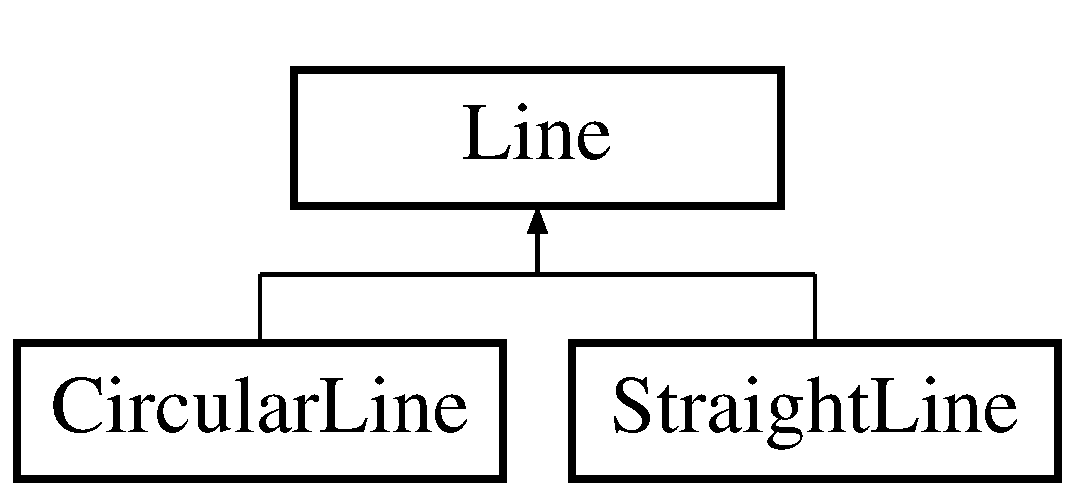
\includegraphics[height=2.000000cm]{class_line}
\end{center}
\end{figure}
\subsection*{Public Member Functions}
\begin{DoxyCompactItemize}
\item 
\mbox{\Hypertarget{class_line_acc11b8a429d8cdd63ba6803dff5602b3}\label{class_line_acc11b8a429d8cdd63ba6803dff5602b3}} 
\mbox{\hyperlink{class_line_acc11b8a429d8cdd63ba6803dff5602b3}{Line}} ()
\begin{DoxyCompactList}\small\item\em constructor of \mbox{\hyperlink{class_line}{Line}} class \end{DoxyCompactList}\item 
\mbox{\hyperlink{class_line_a123e1da8ef560bac5ab6b643e25c3d8f}{Line}} (\mbox{\hyperlink{class_position}{Position}} start\+\_\+point, \mbox{\hyperlink{class_position}{Position}} end\+\_\+point)
\begin{DoxyCompactList}\small\item\em contrusctor of \mbox{\hyperlink{class_line}{Line}} class \end{DoxyCompactList}\item 
\mbox{\Hypertarget{class_line_aabe85f48d22d92b62257091f48174fac}\label{class_line_aabe85f48d22d92b62257091f48174fac}} 
\mbox{\hyperlink{class_line_aabe85f48d22d92b62257091f48174fac}{$\sim$\+Line}} ()
\begin{DoxyCompactList}\small\item\em destructor of the line path \end{DoxyCompactList}\item 
void \mbox{\hyperlink{class_line_a6356eecffc24d5016c9aa697611c3020}{set\+Start\+Point}} (\mbox{\hyperlink{class_position}{Position}} start\+\_\+point\+\_\+i)
\begin{DoxyCompactList}\small\item\em set the start position of the path \end{DoxyCompactList}\item 
\mbox{\hyperlink{class_position}{Position}} \mbox{\hyperlink{class_line_aa9924a540d8ba2da841a414c58dafb56}{get\+Start\+Point}} ()
\begin{DoxyCompactList}\small\item\em return the start point of the path \end{DoxyCompactList}\item 
void \mbox{\hyperlink{class_line_a47359d43675ff78f2b0af8378d952387}{set\+End\+Point}} (\mbox{\hyperlink{class_position}{Position}} end\+\_\+point\+\_\+i)
\begin{DoxyCompactList}\small\item\em set the end point of the path \end{DoxyCompactList}\item 
\mbox{\hyperlink{class_position}{Position}} \mbox{\hyperlink{class_line_a5f22705f0019c1f855f095ea6b7c4b45}{get\+End\+Point}} ()
\begin{DoxyCompactList}\small\item\em return the end point of the path \end{DoxyCompactList}\item 
void \mbox{\hyperlink{class_line_a387afc9536a3c054dec9eb54f45ea993}{set\+Length}} (double length\+\_\+i)
\begin{DoxyCompactList}\small\item\em set the length of the path \end{DoxyCompactList}\item 
double \mbox{\hyperlink{class_line_a9f91895c2a71dcb2c8da5dd5b057b14a}{get\+Length}} ()
\item 
\mbox{\hyperlink{class_position}{Position}} \mbox{\hyperlink{class_line_ad19714c8b94997c96d35fefaa2bbda26}{find\+End\+Point}} (double k, \mbox{\hyperlink{class_position}{Position}} start, double length)
\begin{DoxyCompactList}\small\item\em function that given the curvature the start point and the lenght of the path allow to find the end point of the line \end{DoxyCompactList}\item 
double \mbox{\hyperlink{class_line_a4976ad80d3fe4a789bac7a1916543edd}{sinc}} (double inp)
\begin{DoxyCompactList}\small\item\em Implementation of function sinc(t), returning 1 for t==0, and sin(t)/t. \end{DoxyCompactList}\item 
double \mbox{\hyperlink{class_line_aa30f3bd50c4de544874c4aaad0a24c6a}{mod2pi}} (double ang)
\begin{DoxyCompactList}\small\item\em Normalize an angle (in range \mbox{[}0,2$\ast$pi)) \end{DoxyCompactList}\end{DoxyCompactItemize}


\subsection{Detailed Description}
\mbox{\hyperlink{class_line}{Line}} class that describes the basic line of a path. 

\subsection{Constructor \& Destructor Documentation}
\mbox{\Hypertarget{class_line_a123e1da8ef560bac5ab6b643e25c3d8f}\label{class_line_a123e1da8ef560bac5ab6b643e25c3d8f}} 
\index{Line@{Line}!Line@{Line}}
\index{Line@{Line}!Line@{Line}}
\subsubsection{\texorpdfstring{Line()}{Line()}}
{\footnotesize\ttfamily Line\+::\+Line (\begin{DoxyParamCaption}\item[{\mbox{\hyperlink{class_position}{Position}}}]{start\+\_\+point,  }\item[{\mbox{\hyperlink{class_position}{Position}}}]{end\+\_\+point }\end{DoxyParamCaption})}



contrusctor of \mbox{\hyperlink{class_line}{Line}} class 


\begin{DoxyParams}{Parameters}
{\em start\+\_\+point} & start point of the path \\
\hline
{\em end\+\_\+point} & end point of the path \\
\hline
\end{DoxyParams}


\subsection{Member Function Documentation}
\mbox{\Hypertarget{class_line_ad19714c8b94997c96d35fefaa2bbda26}\label{class_line_ad19714c8b94997c96d35fefaa2bbda26}} 
\index{Line@{Line}!find\+End\+Point@{find\+End\+Point}}
\index{find\+End\+Point@{find\+End\+Point}!Line@{Line}}
\subsubsection{\texorpdfstring{find\+End\+Point()}{findEndPoint()}}
{\footnotesize\ttfamily \mbox{\hyperlink{class_position}{Position}} Line\+::find\+End\+Point (\begin{DoxyParamCaption}\item[{double}]{k,  }\item[{\mbox{\hyperlink{class_position}{Position}}}]{start,  }\item[{double}]{length }\end{DoxyParamCaption})}



function that given the curvature the start point and the lenght of the path allow to find the end point of the line 


\begin{DoxyParams}{Parameters}
{\em k} & curvature \\
\hline
{\em start} & start point of the line \\
\hline
{\em length} & length of the line \\
\hline
\end{DoxyParams}
\begin{DoxyReturn}{Returns}

\end{DoxyReturn}
\mbox{\Hypertarget{class_line_a5f22705f0019c1f855f095ea6b7c4b45}\label{class_line_a5f22705f0019c1f855f095ea6b7c4b45}} 
\index{Line@{Line}!get\+End\+Point@{get\+End\+Point}}
\index{get\+End\+Point@{get\+End\+Point}!Line@{Line}}
\subsubsection{\texorpdfstring{get\+End\+Point()}{getEndPoint()}}
{\footnotesize\ttfamily \mbox{\hyperlink{class_position}{Position}} Line\+::get\+End\+Point (\begin{DoxyParamCaption}{ }\end{DoxyParamCaption})}



return the end point of the path 

\begin{DoxyReturn}{Returns}
the end point of the path 
\end{DoxyReturn}
\mbox{\Hypertarget{class_line_a9f91895c2a71dcb2c8da5dd5b057b14a}\label{class_line_a9f91895c2a71dcb2c8da5dd5b057b14a}} 
\index{Line@{Line}!get\+Length@{get\+Length}}
\index{get\+Length@{get\+Length}!Line@{Line}}
\subsubsection{\texorpdfstring{get\+Length()}{getLength()}}
{\footnotesize\ttfamily double Line\+::get\+Length (\begin{DoxyParamCaption}{ }\end{DoxyParamCaption})}

return the length of the path \begin{DoxyReturn}{Returns}
the length of the path 
\end{DoxyReturn}
\mbox{\Hypertarget{class_line_aa9924a540d8ba2da841a414c58dafb56}\label{class_line_aa9924a540d8ba2da841a414c58dafb56}} 
\index{Line@{Line}!get\+Start\+Point@{get\+Start\+Point}}
\index{get\+Start\+Point@{get\+Start\+Point}!Line@{Line}}
\subsubsection{\texorpdfstring{get\+Start\+Point()}{getStartPoint()}}
{\footnotesize\ttfamily \mbox{\hyperlink{class_position}{Position}} Line\+::get\+Start\+Point (\begin{DoxyParamCaption}{ }\end{DoxyParamCaption})}



return the start point of the path 

\begin{DoxyReturn}{Returns}
the start point 
\end{DoxyReturn}
\mbox{\Hypertarget{class_line_aa30f3bd50c4de544874c4aaad0a24c6a}\label{class_line_aa30f3bd50c4de544874c4aaad0a24c6a}} 
\index{Line@{Line}!mod2pi@{mod2pi}}
\index{mod2pi@{mod2pi}!Line@{Line}}
\subsubsection{\texorpdfstring{mod2pi()}{mod2pi()}}
{\footnotesize\ttfamily double Line\+::mod2pi (\begin{DoxyParamCaption}\item[{double}]{ang }\end{DoxyParamCaption})}



Normalize an angle (in range \mbox{[}0,2$\ast$pi)) 


\begin{DoxyParams}{Parameters}
{\em ang} & input angle \\
\hline
\end{DoxyParams}
\begin{DoxyReturn}{Returns}
the normalize angle in range \mbox{[}0,2$\ast$pi\mbox{]} 
\end{DoxyReturn}
\mbox{\Hypertarget{class_line_a47359d43675ff78f2b0af8378d952387}\label{class_line_a47359d43675ff78f2b0af8378d952387}} 
\index{Line@{Line}!set\+End\+Point@{set\+End\+Point}}
\index{set\+End\+Point@{set\+End\+Point}!Line@{Line}}
\subsubsection{\texorpdfstring{set\+End\+Point()}{setEndPoint()}}
{\footnotesize\ttfamily void Line\+::set\+End\+Point (\begin{DoxyParamCaption}\item[{\mbox{\hyperlink{class_position}{Position}}}]{end\+\_\+point\+\_\+i }\end{DoxyParamCaption})}



set the end point of the path 


\begin{DoxyParams}{Parameters}
{\em end\+\_\+point\+\_\+i} & the end point of the path \\
\hline
\end{DoxyParams}
\mbox{\Hypertarget{class_line_a387afc9536a3c054dec9eb54f45ea993}\label{class_line_a387afc9536a3c054dec9eb54f45ea993}} 
\index{Line@{Line}!set\+Length@{set\+Length}}
\index{set\+Length@{set\+Length}!Line@{Line}}
\subsubsection{\texorpdfstring{set\+Length()}{setLength()}}
{\footnotesize\ttfamily void Line\+::set\+Length (\begin{DoxyParamCaption}\item[{double}]{length\+\_\+i }\end{DoxyParamCaption})}



set the length of the path 


\begin{DoxyParams}{Parameters}
{\em length\+\_\+i} & the length of the path \\
\hline
\end{DoxyParams}
\mbox{\Hypertarget{class_line_a6356eecffc24d5016c9aa697611c3020}\label{class_line_a6356eecffc24d5016c9aa697611c3020}} 
\index{Line@{Line}!set\+Start\+Point@{set\+Start\+Point}}
\index{set\+Start\+Point@{set\+Start\+Point}!Line@{Line}}
\subsubsection{\texorpdfstring{set\+Start\+Point()}{setStartPoint()}}
{\footnotesize\ttfamily void Line\+::set\+Start\+Point (\begin{DoxyParamCaption}\item[{\mbox{\hyperlink{class_position}{Position}}}]{start\+\_\+point\+\_\+i }\end{DoxyParamCaption})}



set the start position of the path 


\begin{DoxyParams}{Parameters}
{\em start\+\_\+point\+\_\+i} & start point of the path \\
\hline
\end{DoxyParams}
\mbox{\Hypertarget{class_line_a4976ad80d3fe4a789bac7a1916543edd}\label{class_line_a4976ad80d3fe4a789bac7a1916543edd}} 
\index{Line@{Line}!sinc@{sinc}}
\index{sinc@{sinc}!Line@{Line}}
\subsubsection{\texorpdfstring{sinc()}{sinc()}}
{\footnotesize\ttfamily double Line\+::sinc (\begin{DoxyParamCaption}\item[{double}]{inp }\end{DoxyParamCaption})}



Implementation of function sinc(t), returning 1 for t==0, and sin(t)/t. 


\begin{DoxyParams}{Parameters}
{\em inp} & input angle \\
\hline
\end{DoxyParams}
\begin{DoxyReturn}{Returns}
1 for inp==0 otherwise sin(inp)/inp 
\end{DoxyReturn}


The documentation for this class was generated from the following file\+:\begin{DoxyCompactItemize}
\item 
Line.\+hpp\end{DoxyCompactItemize}

\hypertarget{class_path}{}\section{Path Class Reference}
\label{class_path}\index{Path@{Path}}
\subsection*{Public Member Functions}
\begin{DoxyCompactItemize}
\item 
\mbox{\hyperlink{class_path_a6abfa12b45ae127daa7408571b62b74d}{Path}} (\mbox{\hyperlink{class_position}{Position}} start\+\_\+point, \mbox{\hyperlink{class_position}{Position}} end\+\_\+point, double curvature, \mbox{\hyperlink{class_map}{Map}} $\ast$map\+\_\+i)
\begin{DoxyCompactList}\small\item\em given the start point and the end point is able to find the best path \end{DoxyCompactList}\item 
\mbox{\Hypertarget{class_path_ab45faf702862c6594068a3ed2d026cda}\label{class_path_ab45faf702862c6594068a3ed2d026cda}} 
void \mbox{\hyperlink{class_path_ab45faf702862c6594068a3ed2d026cda}{find\+Path}} ()
\begin{DoxyCompactList}\small\item\em function that detects the best path, for now uses only dubins path \end{DoxyCompactList}\item 
\mbox{\Hypertarget{class_path_ae5b5816b3480e9f103079bb3467dc65f}\label{class_path_ae5b5816b3480e9f103079bb3467dc65f}} 
void \mbox{\hyperlink{class_path_ae5b5816b3480e9f103079bb3467dc65f}{set\+Lines}} (std\+::vector$<$ \mbox{\hyperlink{class_line}{Line}} $>$)
\begin{DoxyCompactList}\small\item\em set the lines of the path \end{DoxyCompactList}\item 
std\+::vector$<$ \mbox{\hyperlink{class_line}{Line}} $>$ \mbox{\hyperlink{class_path_aff0072e2e1cf183ba6fc240cd85045e2}{get\+Lines}} ()
\begin{DoxyCompactList}\small\item\em return a vector of lines \end{DoxyCompactList}\item 
void \mbox{\hyperlink{class_path_a87f4082a3c5af3aa37260cb99c605156}{set\+Start\+Point}} (\mbox{\hyperlink{class_position}{Position}} start\+\_\+point)
\begin{DoxyCompactList}\small\item\em set the start point of the path \end{DoxyCompactList}\item 
\mbox{\hyperlink{class_position}{Position}} \mbox{\hyperlink{class_path_a88e537e6bfe6140d00b0f36ca642a4cd}{get\+Start\+Point}} ()
\begin{DoxyCompactList}\small\item\em return the start point of the path \end{DoxyCompactList}\item 
void \mbox{\hyperlink{class_path_a168f515818fd9b26a6264fdf95af52e8}{set\+End\+Point}} (\mbox{\hyperlink{class_position}{Position}} end\+\_\+point)
\begin{DoxyCompactList}\small\item\em set the end point of the path \end{DoxyCompactList}\item 
\mbox{\hyperlink{class_position}{Position}} \mbox{\hyperlink{class_path_ac2617080c944b93f7c0c63f3e59aa88c}{get\+End\+Point}} ()
\begin{DoxyCompactList}\small\item\em return the end point of the path \end{DoxyCompactList}\item 
void \mbox{\hyperlink{class_path_a132d54dc6350d1c2eb86611db60df7ff}{set\+Max\+Curvature}} (double curvature)
\begin{DoxyCompactList}\small\item\em set max curvature of the path \end{DoxyCompactList}\item 
double \mbox{\hyperlink{class_path_a613552d171c766462f422593b4957ecc}{get\+Max\+Curvature}} ()
\begin{DoxyCompactList}\small\item\em return of max curvature of the path \end{DoxyCompactList}\item 
void \mbox{\hyperlink{class_path_ad723ba990a07d7542703770a09df52a7}{set\+Length}} (double length)
\begin{DoxyCompactList}\small\item\em set the length of the path \end{DoxyCompactList}\item 
double \mbox{\hyperlink{class_path_ad497d2a12a47bc52a316da83dbe6acbc}{get\+Length}} ()
\begin{DoxyCompactList}\small\item\em return the length of the path \end{DoxyCompactList}\item 
\mbox{\Hypertarget{class_path_a68a50ad6f0fd39d0b272bcb62655b475}\label{class_path_a68a50ad6f0fd39d0b272bcb62655b475}} 
void {\bfseries set\+Map} (\mbox{\hyperlink{class_map}{Map}} $\ast$map\+\_\+i)
\item 
\mbox{\Hypertarget{class_path_abacf46c32c4f36a79c2faf21a9a01270}\label{class_path_abacf46c32c4f36a79c2faf21a9a01270}} 
\mbox{\hyperlink{class_map}{Map}} $\ast$ {\bfseries get\+Map} ()
\end{DoxyCompactItemize}
\subsection*{Public Attributes}
\begin{DoxyCompactItemize}
\item 
\mbox{\Hypertarget{class_path_a822c83d45ed5e336376a813c806ff66b}\label{class_path_a822c83d45ed5e336376a813c806ff66b}} 
\mbox{\hyperlink{class_position}{Position}} {\bfseries start\+\_\+point}
\item 
\mbox{\Hypertarget{class_path_ab97cd4eb2fa1141118bd561c824b27cc}\label{class_path_ab97cd4eb2fa1141118bd561c824b27cc}} 
\mbox{\hyperlink{class_position}{Position}} {\bfseries end\+\_\+point}
\item 
\mbox{\Hypertarget{class_path_a181a2058e947c22fc3e25a361bb934e6}\label{class_path_a181a2058e947c22fc3e25a361bb934e6}} 
double {\bfseries max\+Curvature}
\item 
\mbox{\Hypertarget{class_path_a3d38eb2e010fbf82837e7d3eb5f0faba}\label{class_path_a3d38eb2e010fbf82837e7d3eb5f0faba}} 
std\+::vector$<$ \mbox{\hyperlink{class_line}{Line}} $>$ {\bfseries lines}
\item 
\mbox{\Hypertarget{class_path_a8ca4f648459940bdd347e52f07676473}\label{class_path_a8ca4f648459940bdd347e52f07676473}} 
double {\bfseries length}
\item 
\mbox{\Hypertarget{class_path_a13645419b6b5876ce59368184742b8d7}\label{class_path_a13645419b6b5876ce59368184742b8d7}} 
\mbox{\hyperlink{class_map}{Map}} $\ast$ {\bfseries map}
\end{DoxyCompactItemize}


\subsection{Constructor \& Destructor Documentation}
\mbox{\Hypertarget{class_path_a6abfa12b45ae127daa7408571b62b74d}\label{class_path_a6abfa12b45ae127daa7408571b62b74d}} 
\index{Path@{Path}!Path@{Path}}
\index{Path@{Path}!Path@{Path}}
\subsubsection{\texorpdfstring{Path()}{Path()}}
{\footnotesize\ttfamily Path\+::\+Path (\begin{DoxyParamCaption}\item[{\mbox{\hyperlink{class_position}{Position}}}]{start\+\_\+point,  }\item[{\mbox{\hyperlink{class_position}{Position}}}]{end\+\_\+point,  }\item[{double}]{curvature,  }\item[{\mbox{\hyperlink{class_map}{Map}} $\ast$}]{map\+\_\+i }\end{DoxyParamCaption})}



given the start point and the end point is able to find the best path 


\begin{DoxyParams}{Parameters}
{\em start\+\_\+point} & start point \\
\hline
{\em end\+\_\+point} & end point \\
\hline
\end{DoxyParams}


\subsection{Member Function Documentation}
\mbox{\Hypertarget{class_path_ac2617080c944b93f7c0c63f3e59aa88c}\label{class_path_ac2617080c944b93f7c0c63f3e59aa88c}} 
\index{Path@{Path}!get\+End\+Point@{get\+End\+Point}}
\index{get\+End\+Point@{get\+End\+Point}!Path@{Path}}
\subsubsection{\texorpdfstring{get\+End\+Point()}{getEndPoint()}}
{\footnotesize\ttfamily \mbox{\hyperlink{class_position}{Position}} Path\+::get\+End\+Point (\begin{DoxyParamCaption}{ }\end{DoxyParamCaption})}



return the end point of the path 

\begin{DoxyReturn}{Returns}
the end point of the path 
\end{DoxyReturn}
\mbox{\Hypertarget{class_path_ad497d2a12a47bc52a316da83dbe6acbc}\label{class_path_ad497d2a12a47bc52a316da83dbe6acbc}} 
\index{Path@{Path}!get\+Length@{get\+Length}}
\index{get\+Length@{get\+Length}!Path@{Path}}
\subsubsection{\texorpdfstring{get\+Length()}{getLength()}}
{\footnotesize\ttfamily double Path\+::get\+Length (\begin{DoxyParamCaption}{ }\end{DoxyParamCaption})}



return the length of the path 

\begin{DoxyReturn}{Returns}
the length 

the length 
\end{DoxyReturn}
\mbox{\Hypertarget{class_path_aff0072e2e1cf183ba6fc240cd85045e2}\label{class_path_aff0072e2e1cf183ba6fc240cd85045e2}} 
\index{Path@{Path}!get\+Lines@{get\+Lines}}
\index{get\+Lines@{get\+Lines}!Path@{Path}}
\subsubsection{\texorpdfstring{get\+Lines()}{getLines()}}
{\footnotesize\ttfamily std\+::vector$<$\mbox{\hyperlink{class_line}{Line}}$>$ Path\+::get\+Lines (\begin{DoxyParamCaption}{ }\end{DoxyParamCaption})}



return a vector of lines 

\begin{DoxyReturn}{Returns}
vector of lines 
\end{DoxyReturn}
\mbox{\Hypertarget{class_path_a613552d171c766462f422593b4957ecc}\label{class_path_a613552d171c766462f422593b4957ecc}} 
\index{Path@{Path}!get\+Max\+Curvature@{get\+Max\+Curvature}}
\index{get\+Max\+Curvature@{get\+Max\+Curvature}!Path@{Path}}
\subsubsection{\texorpdfstring{get\+Max\+Curvature()}{getMaxCurvature()}}
{\footnotesize\ttfamily double Path\+::get\+Max\+Curvature (\begin{DoxyParamCaption}{ }\end{DoxyParamCaption})}



return of max curvature of the path 

\begin{DoxyReturn}{Returns}
the max curvature of the path 
\end{DoxyReturn}
\mbox{\Hypertarget{class_path_a88e537e6bfe6140d00b0f36ca642a4cd}\label{class_path_a88e537e6bfe6140d00b0f36ca642a4cd}} 
\index{Path@{Path}!get\+Start\+Point@{get\+Start\+Point}}
\index{get\+Start\+Point@{get\+Start\+Point}!Path@{Path}}
\subsubsection{\texorpdfstring{get\+Start\+Point()}{getStartPoint()}}
{\footnotesize\ttfamily \mbox{\hyperlink{class_position}{Position}} Path\+::get\+Start\+Point (\begin{DoxyParamCaption}{ }\end{DoxyParamCaption})}



return the start point of the path 

\begin{DoxyReturn}{Returns}
the start point of the path 
\end{DoxyReturn}
\mbox{\Hypertarget{class_path_a168f515818fd9b26a6264fdf95af52e8}\label{class_path_a168f515818fd9b26a6264fdf95af52e8}} 
\index{Path@{Path}!set\+End\+Point@{set\+End\+Point}}
\index{set\+End\+Point@{set\+End\+Point}!Path@{Path}}
\subsubsection{\texorpdfstring{set\+End\+Point()}{setEndPoint()}}
{\footnotesize\ttfamily void Path\+::set\+End\+Point (\begin{DoxyParamCaption}\item[{\mbox{\hyperlink{class_position}{Position}}}]{end\+\_\+point }\end{DoxyParamCaption})}



set the end point of the path 


\begin{DoxyParams}{Parameters}
{\em end\+\_\+point} & the end point of the path \\
\hline
\end{DoxyParams}
\mbox{\Hypertarget{class_path_ad723ba990a07d7542703770a09df52a7}\label{class_path_ad723ba990a07d7542703770a09df52a7}} 
\index{Path@{Path}!set\+Length@{set\+Length}}
\index{set\+Length@{set\+Length}!Path@{Path}}
\subsubsection{\texorpdfstring{set\+Length()}{setLength()}}
{\footnotesize\ttfamily void Path\+::set\+Length (\begin{DoxyParamCaption}\item[{double}]{length }\end{DoxyParamCaption})}



set the length of the path 


\begin{DoxyParams}{Parameters}
{\em length} & length of the path \\
\hline
\end{DoxyParams}
\mbox{\Hypertarget{class_path_a132d54dc6350d1c2eb86611db60df7ff}\label{class_path_a132d54dc6350d1c2eb86611db60df7ff}} 
\index{Path@{Path}!set\+Max\+Curvature@{set\+Max\+Curvature}}
\index{set\+Max\+Curvature@{set\+Max\+Curvature}!Path@{Path}}
\subsubsection{\texorpdfstring{set\+Max\+Curvature()}{setMaxCurvature()}}
{\footnotesize\ttfamily void Path\+::set\+Max\+Curvature (\begin{DoxyParamCaption}\item[{double}]{curvature }\end{DoxyParamCaption})}



set max curvature of the path 


\begin{DoxyParams}{Parameters}
{\em curvature} & max curvature of the path \\
\hline
\end{DoxyParams}
\mbox{\Hypertarget{class_path_a87f4082a3c5af3aa37260cb99c605156}\label{class_path_a87f4082a3c5af3aa37260cb99c605156}} 
\index{Path@{Path}!set\+Start\+Point@{set\+Start\+Point}}
\index{set\+Start\+Point@{set\+Start\+Point}!Path@{Path}}
\subsubsection{\texorpdfstring{set\+Start\+Point()}{setStartPoint()}}
{\footnotesize\ttfamily void Path\+::set\+Start\+Point (\begin{DoxyParamCaption}\item[{\mbox{\hyperlink{class_position}{Position}}}]{start\+\_\+point }\end{DoxyParamCaption})}



set the start point of the path 


\begin{DoxyParams}{Parameters}
{\em start\+\_\+point} & start point of the path \\
\hline
\end{DoxyParams}


The documentation for this class was generated from the following file\+:\begin{DoxyCompactItemize}
\item 
Path.\+hpp\end{DoxyCompactItemize}

\hypertarget{class_path_coordinates}{}\section{Path\+Coordinates Class Reference}
\label{class_path_coordinates}\index{Path\+Coordinates@{Path\+Coordinates}}


class for storing data that describes the path  




{\ttfamily \#include $<$Path\+Coordinates.\+hpp$>$}

\subsection*{Public Member Functions}
\begin{DoxyCompactItemize}
\item 
\mbox{\hyperlink{class_path_coordinates_a6540a40d24cb4e50577eda489b7fe1bb}{Path\+Coordinates}} (\mbox{\hyperlink{class_position}{Position}} position\+\_\+in, \mbox{\hyperlink{class_position}{Position}} position\+\_\+fin, double curvature\+\_\+p)
\begin{DoxyCompactList}\small\item\em constructor of the \mbox{\hyperlink{class_path_coordinates}{Path\+Coordinates}} class \end{DoxyCompactList}\item 
\mbox{\Hypertarget{class_path_coordinates_a960c365c8307fb139e425a24d2eb8c66}\label{class_path_coordinates_a960c365c8307fb139e425a24d2eb8c66}} 
\mbox{\hyperlink{class_path_coordinates_a960c365c8307fb139e425a24d2eb8c66}{$\sim$\+Path\+Coordinates}} ()
\begin{DoxyCompactList}\small\item\em destructor of the \mbox{\hyperlink{class_path_coordinates}{Path\+Coordinates}} class \end{DoxyCompactList}\item 
void \mbox{\hyperlink{class_path_coordinates_a730ba85010cbd33da4e76fe0f05fb2b0}{set\+Positions}} (\mbox{\hyperlink{class_position}{Position}} position\+\_\+in, \mbox{\hyperlink{class_position}{Position}} position\+\_\+fin)
\item 
\mbox{\hyperlink{class_position}{Position}} \mbox{\hyperlink{class_path_coordinates_a10450bb899bec6d9f8be0a115c2c588b}{get\+Initial\+Position}} ()
\begin{DoxyCompactList}\small\item\em return the initial position of the path \end{DoxyCompactList}\item 
\mbox{\hyperlink{class_position}{Position}} \mbox{\hyperlink{class_path_coordinates_af4d85fae7c4ed67ea5201895d1ee4b7b}{get\+Final\+Position}} ()
\begin{DoxyCompactList}\small\item\em return the final position of the path \end{DoxyCompactList}\item 
double \mbox{\hyperlink{class_path_coordinates_a6b0315b737b35af2e198a7094828741e}{get\+Max\+Curvature}} ()
\begin{DoxyCompactList}\small\item\em return the curvature of the path \end{DoxyCompactList}\item 
void \mbox{\hyperlink{class_path_coordinates_abd7e9a8143e368f9290b962f595ae0a8}{set\+Max\+Curvature}} (double curvature\+\_\+p)
\begin{DoxyCompactList}\small\item\em set the max curvature of the path \end{DoxyCompactList}\end{DoxyCompactItemize}


\subsection{Detailed Description}
class for storing data that describes the path 

\subsection{Constructor \& Destructor Documentation}
\mbox{\Hypertarget{class_path_coordinates_a6540a40d24cb4e50577eda489b7fe1bb}\label{class_path_coordinates_a6540a40d24cb4e50577eda489b7fe1bb}} 
\index{Path\+Coordinates@{Path\+Coordinates}!Path\+Coordinates@{Path\+Coordinates}}
\index{Path\+Coordinates@{Path\+Coordinates}!Path\+Coordinates@{Path\+Coordinates}}
\subsubsection{\texorpdfstring{Path\+Coordinates()}{PathCoordinates()}}
{\footnotesize\ttfamily Path\+Coordinates\+::\+Path\+Coordinates (\begin{DoxyParamCaption}\item[{\mbox{\hyperlink{class_position}{Position}}}]{position\+\_\+in,  }\item[{\mbox{\hyperlink{class_position}{Position}}}]{position\+\_\+fin,  }\item[{double}]{curvature\+\_\+p }\end{DoxyParamCaption})}



constructor of the \mbox{\hyperlink{class_path_coordinates}{Path\+Coordinates}} class 


\begin{DoxyParams}{Parameters}
{\em position\+\_\+in} & initial position of the path \\
\hline
{\em position\+\_\+fin} & final position if the path \\
\hline
{\em curvature\+\_\+p} & curvature of the path \\
\hline
\end{DoxyParams}


\subsection{Member Function Documentation}
\mbox{\Hypertarget{class_path_coordinates_af4d85fae7c4ed67ea5201895d1ee4b7b}\label{class_path_coordinates_af4d85fae7c4ed67ea5201895d1ee4b7b}} 
\index{Path\+Coordinates@{Path\+Coordinates}!get\+Final\+Position@{get\+Final\+Position}}
\index{get\+Final\+Position@{get\+Final\+Position}!Path\+Coordinates@{Path\+Coordinates}}
\subsubsection{\texorpdfstring{get\+Final\+Position()}{getFinalPosition()}}
{\footnotesize\ttfamily \mbox{\hyperlink{class_position}{Position}} Path\+Coordinates\+::get\+Final\+Position (\begin{DoxyParamCaption}{ }\end{DoxyParamCaption})}



return the final position of the path 

\begin{DoxyReturn}{Returns}
the final position of the path 
\end{DoxyReturn}
\mbox{\Hypertarget{class_path_coordinates_a10450bb899bec6d9f8be0a115c2c588b}\label{class_path_coordinates_a10450bb899bec6d9f8be0a115c2c588b}} 
\index{Path\+Coordinates@{Path\+Coordinates}!get\+Initial\+Position@{get\+Initial\+Position}}
\index{get\+Initial\+Position@{get\+Initial\+Position}!Path\+Coordinates@{Path\+Coordinates}}
\subsubsection{\texorpdfstring{get\+Initial\+Position()}{getInitialPosition()}}
{\footnotesize\ttfamily \mbox{\hyperlink{class_position}{Position}} Path\+Coordinates\+::get\+Initial\+Position (\begin{DoxyParamCaption}{ }\end{DoxyParamCaption})}



return the initial position of the path 

\begin{DoxyReturn}{Returns}
the initial position of the path 
\end{DoxyReturn}
\mbox{\Hypertarget{class_path_coordinates_a6b0315b737b35af2e198a7094828741e}\label{class_path_coordinates_a6b0315b737b35af2e198a7094828741e}} 
\index{Path\+Coordinates@{Path\+Coordinates}!get\+Max\+Curvature@{get\+Max\+Curvature}}
\index{get\+Max\+Curvature@{get\+Max\+Curvature}!Path\+Coordinates@{Path\+Coordinates}}
\subsubsection{\texorpdfstring{get\+Max\+Curvature()}{getMaxCurvature()}}
{\footnotesize\ttfamily double Path\+Coordinates\+::get\+Max\+Curvature (\begin{DoxyParamCaption}{ }\end{DoxyParamCaption})}



return the curvature of the path 

\begin{DoxyReturn}{Returns}
the curvature of the path 
\end{DoxyReturn}
\mbox{\Hypertarget{class_path_coordinates_abd7e9a8143e368f9290b962f595ae0a8}\label{class_path_coordinates_abd7e9a8143e368f9290b962f595ae0a8}} 
\index{Path\+Coordinates@{Path\+Coordinates}!set\+Max\+Curvature@{set\+Max\+Curvature}}
\index{set\+Max\+Curvature@{set\+Max\+Curvature}!Path\+Coordinates@{Path\+Coordinates}}
\subsubsection{\texorpdfstring{set\+Max\+Curvature()}{setMaxCurvature()}}
{\footnotesize\ttfamily void Path\+Coordinates\+::set\+Max\+Curvature (\begin{DoxyParamCaption}\item[{double}]{curvature\+\_\+p }\end{DoxyParamCaption})}



set the max curvature of the path 


\begin{DoxyParams}{Parameters}
{\em curvature\+\_\+p} & the max curvature of the path \\
\hline
\end{DoxyParams}
\mbox{\Hypertarget{class_path_coordinates_a730ba85010cbd33da4e76fe0f05fb2b0}\label{class_path_coordinates_a730ba85010cbd33da4e76fe0f05fb2b0}} 
\index{Path\+Coordinates@{Path\+Coordinates}!set\+Positions@{set\+Positions}}
\index{set\+Positions@{set\+Positions}!Path\+Coordinates@{Path\+Coordinates}}
\subsubsection{\texorpdfstring{set\+Positions()}{setPositions()}}
{\footnotesize\ttfamily void Path\+Coordinates\+::set\+Positions (\begin{DoxyParamCaption}\item[{\mbox{\hyperlink{class_position}{Position}}}]{position\+\_\+in,  }\item[{\mbox{\hyperlink{class_position}{Position}}}]{position\+\_\+fin }\end{DoxyParamCaption})}

set the initial and the final position of the path 
\begin{DoxyParams}{Parameters}
{\em position\+\_\+in} & initial position of the path \\
\hline
{\em position\+\_\+fin} & final position of the path \\
\hline
\end{DoxyParams}


The documentation for this class was generated from the following file\+:\begin{DoxyCompactItemize}
\item 
Path\+Coordinates.\+hpp\end{DoxyCompactItemize}

\hypertarget{class_position}{}\section{Position Class Reference}
\label{class_position}\index{Position@{Position}}


describes a position of a point using x and y coordinates and orientation  




{\ttfamily \#include $<$Position.\+hpp$>$}

\subsection*{Public Member Functions}
\begin{DoxyCompactItemize}
\item 
\mbox{\Hypertarget{class_position_a369a577425f8ba02e8750d04b6a088db}\label{class_position_a369a577425f8ba02e8750d04b6a088db}} 
\mbox{\hyperlink{class_position_a369a577425f8ba02e8750d04b6a088db}{Position}} ()
\begin{DoxyCompactList}\small\item\em constructor of the \mbox{\hyperlink{class_position}{Position}} class \end{DoxyCompactList}\item 
\mbox{\hyperlink{class_position_adafef18a82e49bf4c91ff0a31b82ff05}{Position}} (cv\+::\+Point2d pos, double orient)
\begin{DoxyCompactList}\small\item\em constructor of the \mbox{\hyperlink{class_position}{Position}} class \end{DoxyCompactList}\item 
\mbox{\Hypertarget{class_position_abe83df4cab7af756636b4e39e4378f4a}\label{class_position_abe83df4cab7af756636b4e39e4378f4a}} 
\mbox{\hyperlink{class_position_abe83df4cab7af756636b4e39e4378f4a}{$\sim$\+Position}} ()
\begin{DoxyCompactList}\small\item\em destructor of the \mbox{\hyperlink{class_position}{Position}} class \end{DoxyCompactList}\item 
void \mbox{\hyperlink{class_position_acf00d240f456cc9b2c2910e803f53605}{set\+Position}} (cv\+::\+Point2d position\+\_\+p, double orientation\+\_\+p)
\begin{DoxyCompactList}\small\item\em set the values of the position \end{DoxyCompactList}\item 
cv\+::\+Point2d \mbox{\hyperlink{class_position_a9de96881a3ea441b4cfb26339172dc6f}{get\+Coordinates}} ()
\begin{DoxyCompactList}\small\item\em return the coordinates of the position \end{DoxyCompactList}\item 
double \mbox{\hyperlink{class_position_af0b1158a379d54dd7ee08164eafe262e}{get\+Orientation}} ()
\begin{DoxyCompactList}\small\item\em return the orientation of the position \end{DoxyCompactList}\end{DoxyCompactItemize}
\subsection*{Public Attributes}
\begin{DoxyCompactItemize}
\item 
\mbox{\Hypertarget{class_position_abdbf5ff8fe616dbc3c9381fce3758845}\label{class_position_abdbf5ff8fe616dbc3c9381fce3758845}} 
bool {\bfseries orientation\+\_\+locked} = false
\item 
\mbox{\Hypertarget{class_position_ad31b8c464b0cee9201cf39f395eb365f}\label{class_position_ad31b8c464b0cee9201cf39f395eb365f}} 
double {\bfseries orientation}
\end{DoxyCompactItemize}


\subsection{Detailed Description}
describes a position of a point using x and y coordinates and orientation 

\subsection{Constructor \& Destructor Documentation}
\mbox{\Hypertarget{class_position_adafef18a82e49bf4c91ff0a31b82ff05}\label{class_position_adafef18a82e49bf4c91ff0a31b82ff05}} 
\index{Position@{Position}!Position@{Position}}
\index{Position@{Position}!Position@{Position}}
\subsubsection{\texorpdfstring{Position()}{Position()}}
{\footnotesize\ttfamily Position\+::\+Position (\begin{DoxyParamCaption}\item[{cv\+::\+Point2d}]{pos,  }\item[{double}]{orient }\end{DoxyParamCaption})}



constructor of the \mbox{\hyperlink{class_position}{Position}} class 


\begin{DoxyParams}{Parameters}
{\em pos} & x and y coordinates \\
\hline
{\em orient} & orientation \\
\hline
\end{DoxyParams}


\subsection{Member Function Documentation}
\mbox{\Hypertarget{class_position_a9de96881a3ea441b4cfb26339172dc6f}\label{class_position_a9de96881a3ea441b4cfb26339172dc6f}} 
\index{Position@{Position}!get\+Coordinates@{get\+Coordinates}}
\index{get\+Coordinates@{get\+Coordinates}!Position@{Position}}
\subsubsection{\texorpdfstring{get\+Coordinates()}{getCoordinates()}}
{\footnotesize\ttfamily cv\+::\+Point2d Position\+::get\+Coordinates (\begin{DoxyParamCaption}{ }\end{DoxyParamCaption})}



return the coordinates of the position 

\begin{DoxyReturn}{Returns}
the coordinates of the position 
\end{DoxyReturn}
\mbox{\Hypertarget{class_position_af0b1158a379d54dd7ee08164eafe262e}\label{class_position_af0b1158a379d54dd7ee08164eafe262e}} 
\index{Position@{Position}!get\+Orientation@{get\+Orientation}}
\index{get\+Orientation@{get\+Orientation}!Position@{Position}}
\subsubsection{\texorpdfstring{get\+Orientation()}{getOrientation()}}
{\footnotesize\ttfamily double Position\+::get\+Orientation (\begin{DoxyParamCaption}{ }\end{DoxyParamCaption})}



return the orientation of the position 

\begin{DoxyReturn}{Returns}
the orientation of the position 
\end{DoxyReturn}
\mbox{\Hypertarget{class_position_acf00d240f456cc9b2c2910e803f53605}\label{class_position_acf00d240f456cc9b2c2910e803f53605}} 
\index{Position@{Position}!set\+Position@{set\+Position}}
\index{set\+Position@{set\+Position}!Position@{Position}}
\subsubsection{\texorpdfstring{set\+Position()}{setPosition()}}
{\footnotesize\ttfamily void Position\+::set\+Position (\begin{DoxyParamCaption}\item[{cv\+::\+Point2d}]{position\+\_\+p,  }\item[{double}]{orientation\+\_\+p }\end{DoxyParamCaption})}



set the values of the position 


\begin{DoxyParams}{Parameters}
{\em position\+\_\+p} & coordinates \\
\hline
{\em orientation\+\_\+p} & orientation \\
\hline
\end{DoxyParams}


The documentation for this class was generated from the following file\+:\begin{DoxyCompactItemize}
\item 
Position.\+hpp\end{DoxyCompactItemize}

\hypertarget{class_possible_dubin_path}{}\section{Possible\+Dubin\+Path Class Reference}
\label{class_possible_dubin_path}\index{Possible\+Dubin\+Path@{Possible\+Dubin\+Path}}


class that describes a possible dubin path (useful during the calculation)  




{\ttfamily \#include $<$Possible\+Dubin\+Path.\+hpp$>$}

\subsection*{Public Member Functions}
\begin{DoxyCompactItemize}
\item 
\mbox{\Hypertarget{class_possible_dubin_path_a1b5581a6922da0c296bb3101081e64fe}\label{class_possible_dubin_path_a1b5581a6922da0c296bb3101081e64fe}} 
\mbox{\hyperlink{class_possible_dubin_path_a1b5581a6922da0c296bb3101081e64fe}{Possible\+Dubin\+Path}} ()
\begin{DoxyCompactList}\small\item\em constructor of \mbox{\hyperlink{class_possible_dubin_path}{Possible\+Dubin\+Path}} class \end{DoxyCompactList}\item 
\mbox{\Hypertarget{class_possible_dubin_path_a6fdb36aaf60e69133e99511fe2abed4d}\label{class_possible_dubin_path_a6fdb36aaf60e69133e99511fe2abed4d}} 
\mbox{\hyperlink{class_possible_dubin_path_a6fdb36aaf60e69133e99511fe2abed4d}{$\sim$\+Possible\+Dubin\+Path}} ()
\begin{DoxyCompactList}\small\item\em destructor of \mbox{\hyperlink{class_possible_dubin_path}{Possible\+Dubin\+Path}} class \end{DoxyCompactList}\end{DoxyCompactItemize}
\subsection*{Public Attributes}
\begin{DoxyCompactItemize}
\item 
\mbox{\Hypertarget{class_possible_dubin_path_afc163a7191f0f0ef7f3ab9e4b9f0475a}\label{class_possible_dubin_path_afc163a7191f0f0ef7f3ab9e4b9f0475a}} 
bool {\bfseries ok}
\item 
\mbox{\Hypertarget{class_possible_dubin_path_a30080622e0aa5d77e9bd4e48ce899fd3}\label{class_possible_dubin_path_a30080622e0aa5d77e9bd4e48ce899fd3}} 
double {\bfseries sc\+\_\+s1}
\item 
\mbox{\Hypertarget{class_possible_dubin_path_a7718b2c4e85c79af611e9730cf64e5c7}\label{class_possible_dubin_path_a7718b2c4e85c79af611e9730cf64e5c7}} 
double {\bfseries sc\+\_\+s2}
\item 
\mbox{\Hypertarget{class_possible_dubin_path_a158d88da33832122490ad12569f656d9}\label{class_possible_dubin_path_a158d88da33832122490ad12569f656d9}} 
double {\bfseries sc\+\_\+s3}
\item 
\mbox{\Hypertarget{class_possible_dubin_path_a32c2b643e10f119657c1a682c9e8c774}\label{class_possible_dubin_path_a32c2b643e10f119657c1a682c9e8c774}} 
std\+::vector$<$ int $>$ {\bfseries signs}
\end{DoxyCompactItemize}


\subsection{Detailed Description}
class that describes a possible dubin path (useful during the calculation) 

The documentation for this class was generated from the following file\+:\begin{DoxyCompactItemize}
\item 
Possible\+Dubin\+Path.\+hpp\end{DoxyCompactItemize}

\hypertarget{structstandard_conf}{}\section{standard\+Conf Struct Reference}
\label{structstandard_conf}\index{standard\+Conf@{standard\+Conf}}
\subsection*{Public Attributes}
\begin{DoxyCompactItemize}
\item 
\mbox{\Hypertarget{structstandard_conf_ac5a8976654eddd1c14b2aab5f4401943}\label{structstandard_conf_ac5a8976654eddd1c14b2aab5f4401943}} 
double {\bfseries lambda}
\item 
\mbox{\Hypertarget{structstandard_conf_a105f1c9c8b50dc1f82ded42d04efeddb}\label{structstandard_conf_a105f1c9c8b50dc1f82ded42d04efeddb}} 
double {\bfseries sc\+\_\+th0}
\item 
\mbox{\Hypertarget{structstandard_conf_a10bf9ad5cc1f29e5414bcad2d762273c}\label{structstandard_conf_a10bf9ad5cc1f29e5414bcad2d762273c}} 
double {\bfseries sc\+\_\+thf}
\item 
\mbox{\Hypertarget{structstandard_conf_a394472a69fcea7d55ff5925a878e4d2d}\label{structstandard_conf_a394472a69fcea7d55ff5925a878e4d2d}} 
double {\bfseries sc\+\_\+\+Kmax}
\end{DoxyCompactItemize}


The documentation for this struct was generated from the following file\+:\begin{DoxyCompactItemize}
\item 
Dubin\+Path\+Finder.\+hpp\end{DoxyCompactItemize}

\hypertarget{class_straight_line}{}\section{Straight\+Line Class Reference}
\label{class_straight_line}\index{Straight\+Line@{Straight\+Line}}


describe a \mbox{\hyperlink{class_straight_line}{Straight\+Line}} in the path  




{\ttfamily \#include $<$Straight\+Line.\+hpp$>$}

Inheritance diagram for Straight\+Line\+:\begin{figure}[H]
\begin{center}
\leavevmode
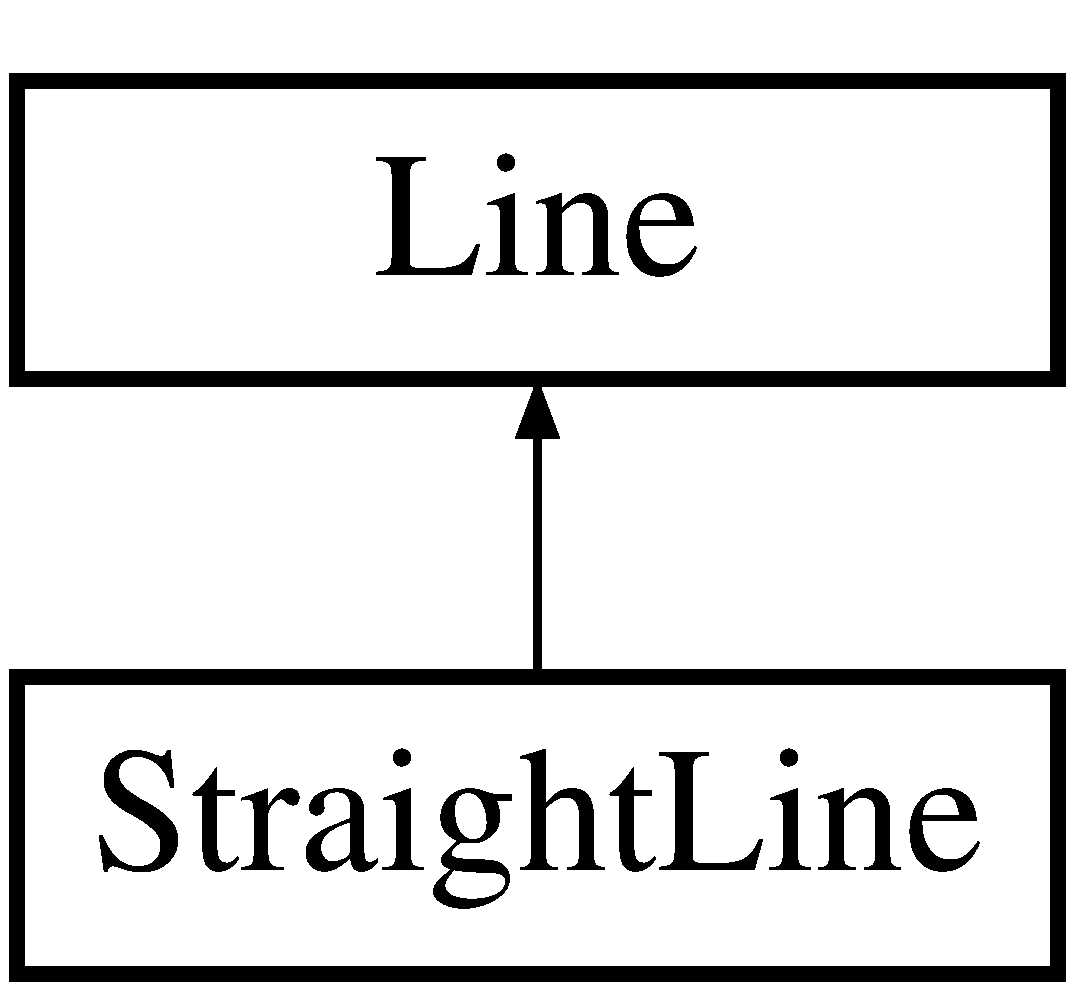
\includegraphics[height=2.000000cm]{class_straight_line}
\end{center}
\end{figure}
\subsection*{Public Member Functions}
\begin{DoxyCompactItemize}
\item 
\mbox{\hyperlink{class_straight_line_a583064766a4c73bfa58ee1cb9f5b4495}{Straight\+Line}} (\mbox{\hyperlink{class_position}{Position}} start\+\_\+point, \mbox{\hyperlink{class_position}{Position}} end\+\_\+point)
\begin{DoxyCompactList}\small\item\em constructor of the \mbox{\hyperlink{class_straight_line}{Straight\+Line}} class \end{DoxyCompactList}\item 
\mbox{\hyperlink{class_straight_line_ac55a20f7c9d8ba62f4dd0bba0e9d8c4e}{Straight\+Line}} (\mbox{\hyperlink{class_position}{Position}} start\+\_\+point, double length)
\begin{DoxyCompactList}\small\item\em constructor of the \mbox{\hyperlink{class_straight_line}{Straight\+Line}} class \end{DoxyCompactList}\item 
\mbox{\Hypertarget{class_straight_line_a24fc4b7e915d5a42b40f716e49558663}\label{class_straight_line_a24fc4b7e915d5a42b40f716e49558663}} 
\mbox{\hyperlink{class_straight_line_a24fc4b7e915d5a42b40f716e49558663}{$\sim$\+Straight\+Line}} ()
\begin{DoxyCompactList}\small\item\em destructor of the \mbox{\hyperlink{class_straight_line}{Straight\+Line}} class \end{DoxyCompactList}\end{DoxyCompactItemize}


\subsection{Detailed Description}
describe a \mbox{\hyperlink{class_straight_line}{Straight\+Line}} in the path 

\subsection{Constructor \& Destructor Documentation}
\mbox{\Hypertarget{class_straight_line_a583064766a4c73bfa58ee1cb9f5b4495}\label{class_straight_line_a583064766a4c73bfa58ee1cb9f5b4495}} 
\index{Straight\+Line@{Straight\+Line}!Straight\+Line@{Straight\+Line}}
\index{Straight\+Line@{Straight\+Line}!Straight\+Line@{Straight\+Line}}
\subsubsection{\texorpdfstring{Straight\+Line()}{StraightLine()}\hspace{0.1cm}{\footnotesize\ttfamily [1/2]}}
{\footnotesize\ttfamily Straight\+Line\+::\+Straight\+Line (\begin{DoxyParamCaption}\item[{\mbox{\hyperlink{class_position}{Position}}}]{start\+\_\+point,  }\item[{\mbox{\hyperlink{class_position}{Position}}}]{end\+\_\+point }\end{DoxyParamCaption})}



constructor of the \mbox{\hyperlink{class_straight_line}{Straight\+Line}} class 


\begin{DoxyParams}{Parameters}
{\em start\+\_\+point} & start point of the line \\
\hline
{\em end\+\_\+point} & end point of the line \\
\hline
\end{DoxyParams}
\mbox{\Hypertarget{class_straight_line_ac55a20f7c9d8ba62f4dd0bba0e9d8c4e}\label{class_straight_line_ac55a20f7c9d8ba62f4dd0bba0e9d8c4e}} 
\index{Straight\+Line@{Straight\+Line}!Straight\+Line@{Straight\+Line}}
\index{Straight\+Line@{Straight\+Line}!Straight\+Line@{Straight\+Line}}
\subsubsection{\texorpdfstring{Straight\+Line()}{StraightLine()}\hspace{0.1cm}{\footnotesize\ttfamily [2/2]}}
{\footnotesize\ttfamily Straight\+Line\+::\+Straight\+Line (\begin{DoxyParamCaption}\item[{\mbox{\hyperlink{class_position}{Position}}}]{start\+\_\+point,  }\item[{double}]{length }\end{DoxyParamCaption})}



constructor of the \mbox{\hyperlink{class_straight_line}{Straight\+Line}} class 


\begin{DoxyParams}{Parameters}
{\em start\+\_\+point} & start point of the line \\
\hline
{\em length} & length of the line \\
\hline
\end{DoxyParams}


The documentation for this class was generated from the following file\+:\begin{DoxyCompactItemize}
\item 
Straight\+Line.\+hpp\end{DoxyCompactItemize}

%--- End generated contents ---

% Index
\backmatter
\newpage
\phantomsection
\clearemptydoublepage
\addcontentsline{toc}{chapter}{Index}
\printindex

\end{document}
